\chapter{Background}
\label{ch:background}
This chapter gives background information about the robots used for the experiments, the OCU used to communicate with the robots, the software running on the robots and the area used for testing.

For the robots to drive around on their own all they require is an estimate of where they are, a path to follow, a controller to determine the actuator outputs and motor controllers to perform the controller outputs.

\section{Small Unmanned Ground Vehicles}
\label{sec:smallugvs}
There are two commonly used robots in EOD applications, the iRobot Packbot and Kinetiq Talon, which are differential drive robots with two motors that drive tracks on either side of the robot. These two robots were used in the experiments that follow. Additionally, the Urbot (developed by SPAWAR Systems Center, Pacific (SSCPAC)) and the Autonomous Solutions Chaos robots were tested. The OCU and software developed for estimation, planning and controls runs on all four robots although most of the testing was done using a Packbot. Note that differential drive, skid steer and unicycle-like robots are synonymous descriptions in the literature and used interchangeably in this thesis.

Each of the robots has a computer that accepts teleoperation commands consisting of a linear and angular velocity. Additionally, each robot has a payload bay where another computer and sensors used for autonomous navigation are located. The payload computer is used to read sensor data and calculate appropriate linear and angular velocity commands that are sent to the robot computer. The standard sensors available on each robot are a gyro, wheel encoders, inertial measurement unit (IMU) and a global position system (GPS) receiver.

The \href{http://www.irobot.com/sp.cfm?pageid=171}{Packbot} is manufactured by iRobot and can be seen in Figure \ref{fig:packbot}.

\begin{figure}[ht!]
	\centering
	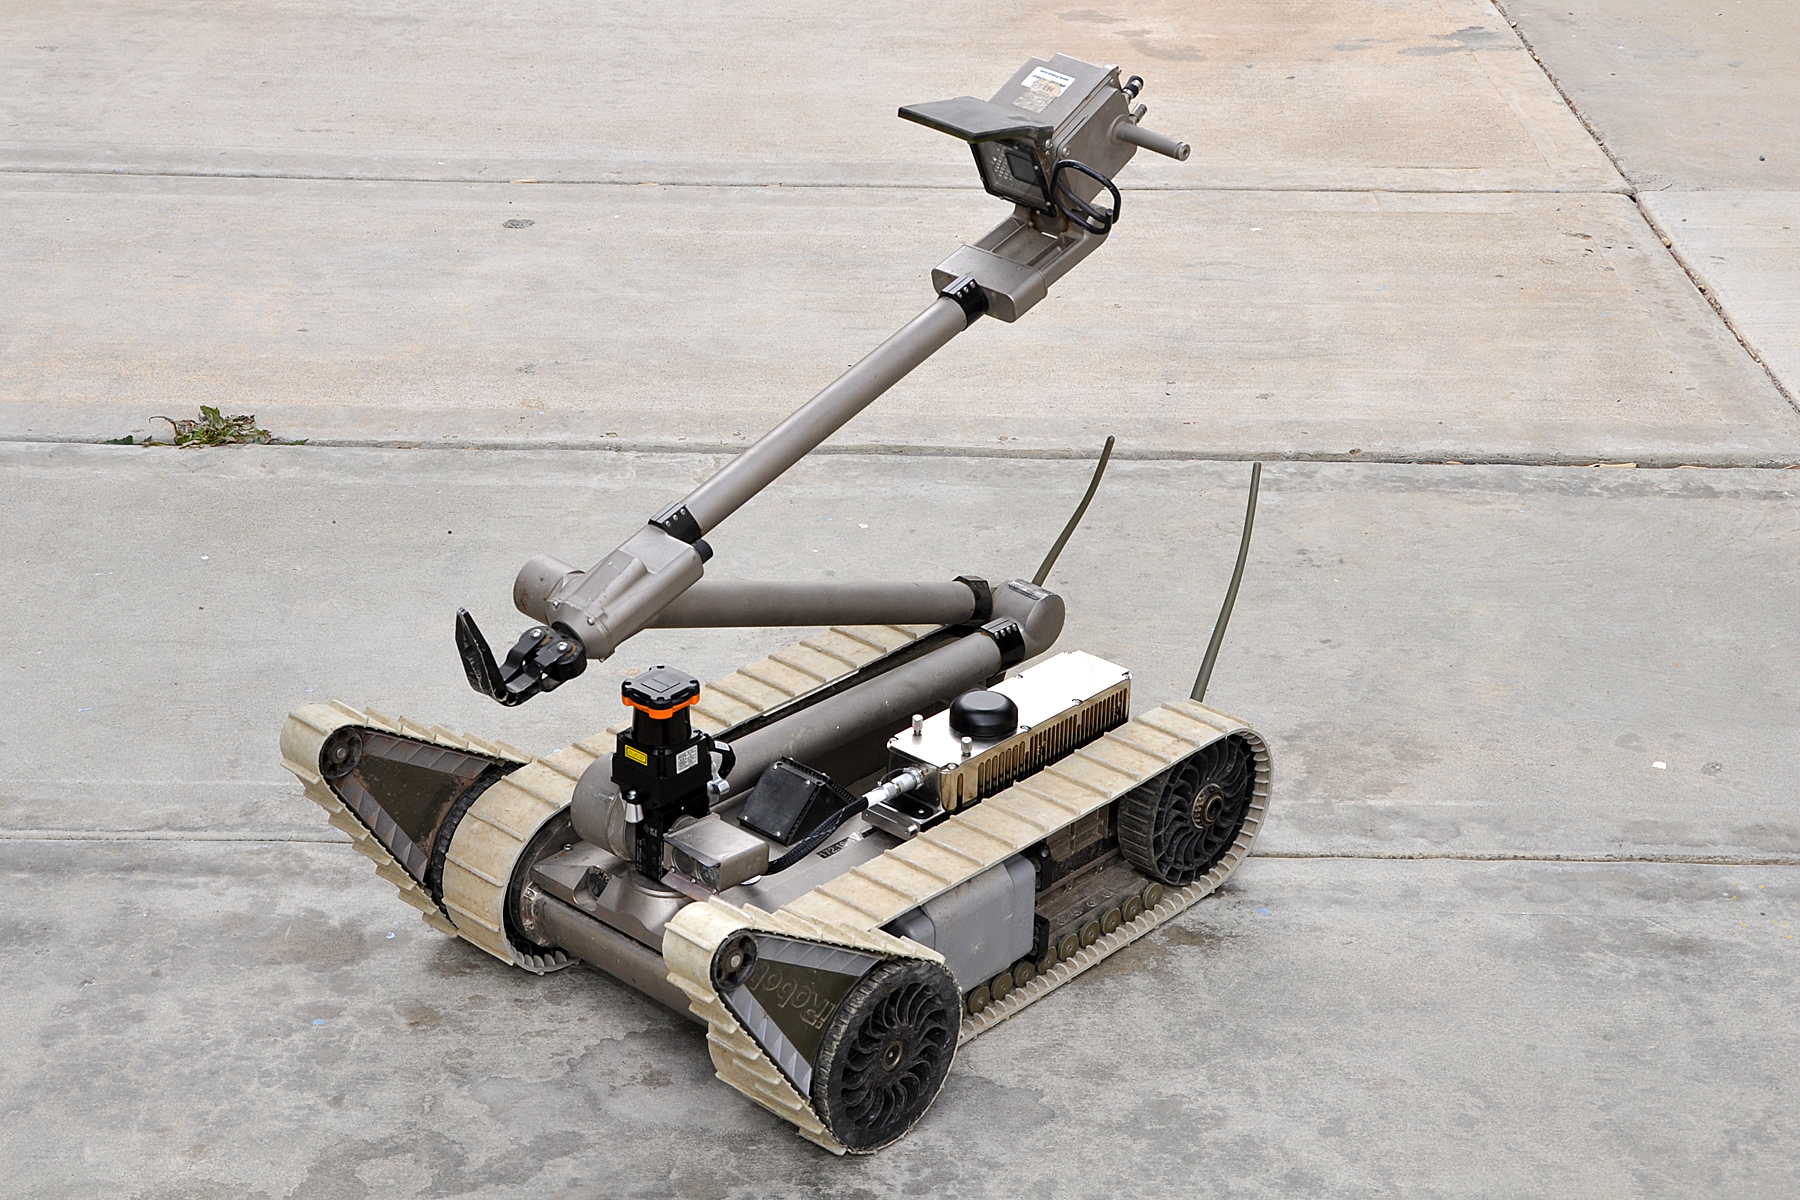
\includegraphics[width=.3\textwidth]{images/packbotRetrotraverse}
	\caption{iRobot Packbot}
	\label{fig:packbot}
\end{figure}

The \href{http://www.foster-miller.com/lemming.htm}{Talon} is manufactured by Kinetiq and is shown in Figure \ref{fig:talon}.

\begin{figure}[ht!]
	\centering
	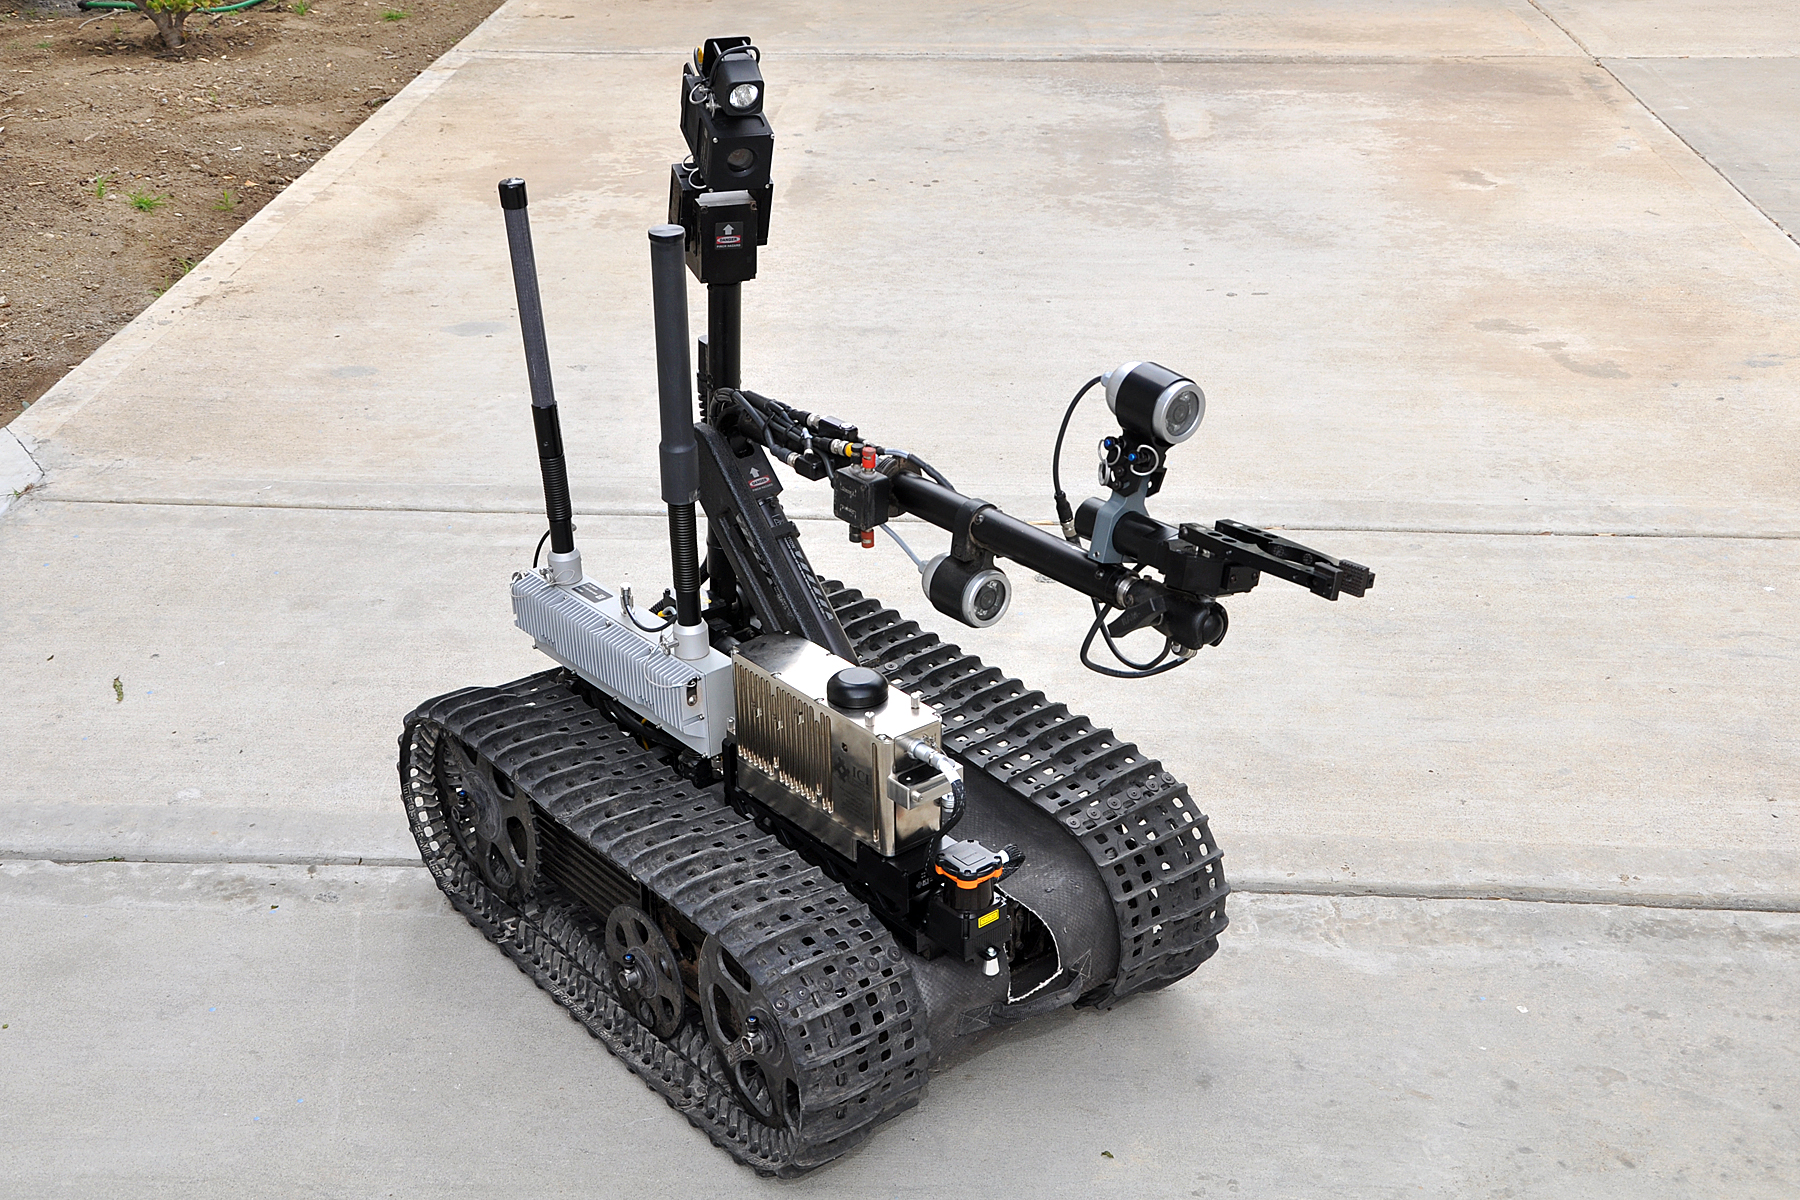
\includegraphics[width=.3\textwidth]{images/talonRetrotraverse}
	\caption{Kinetiq Talon}
	\label{fig:talon}
\end{figure}

The \href{http://www.spawar.navy.mil/robots/land/mprs/mprs.html}{Urbot} is an experimental prototype of a small robot developed by SSCPAC and is shown in Figure \ref{fig:urbot}.

\begin{figure}[ht!]
	\centering
	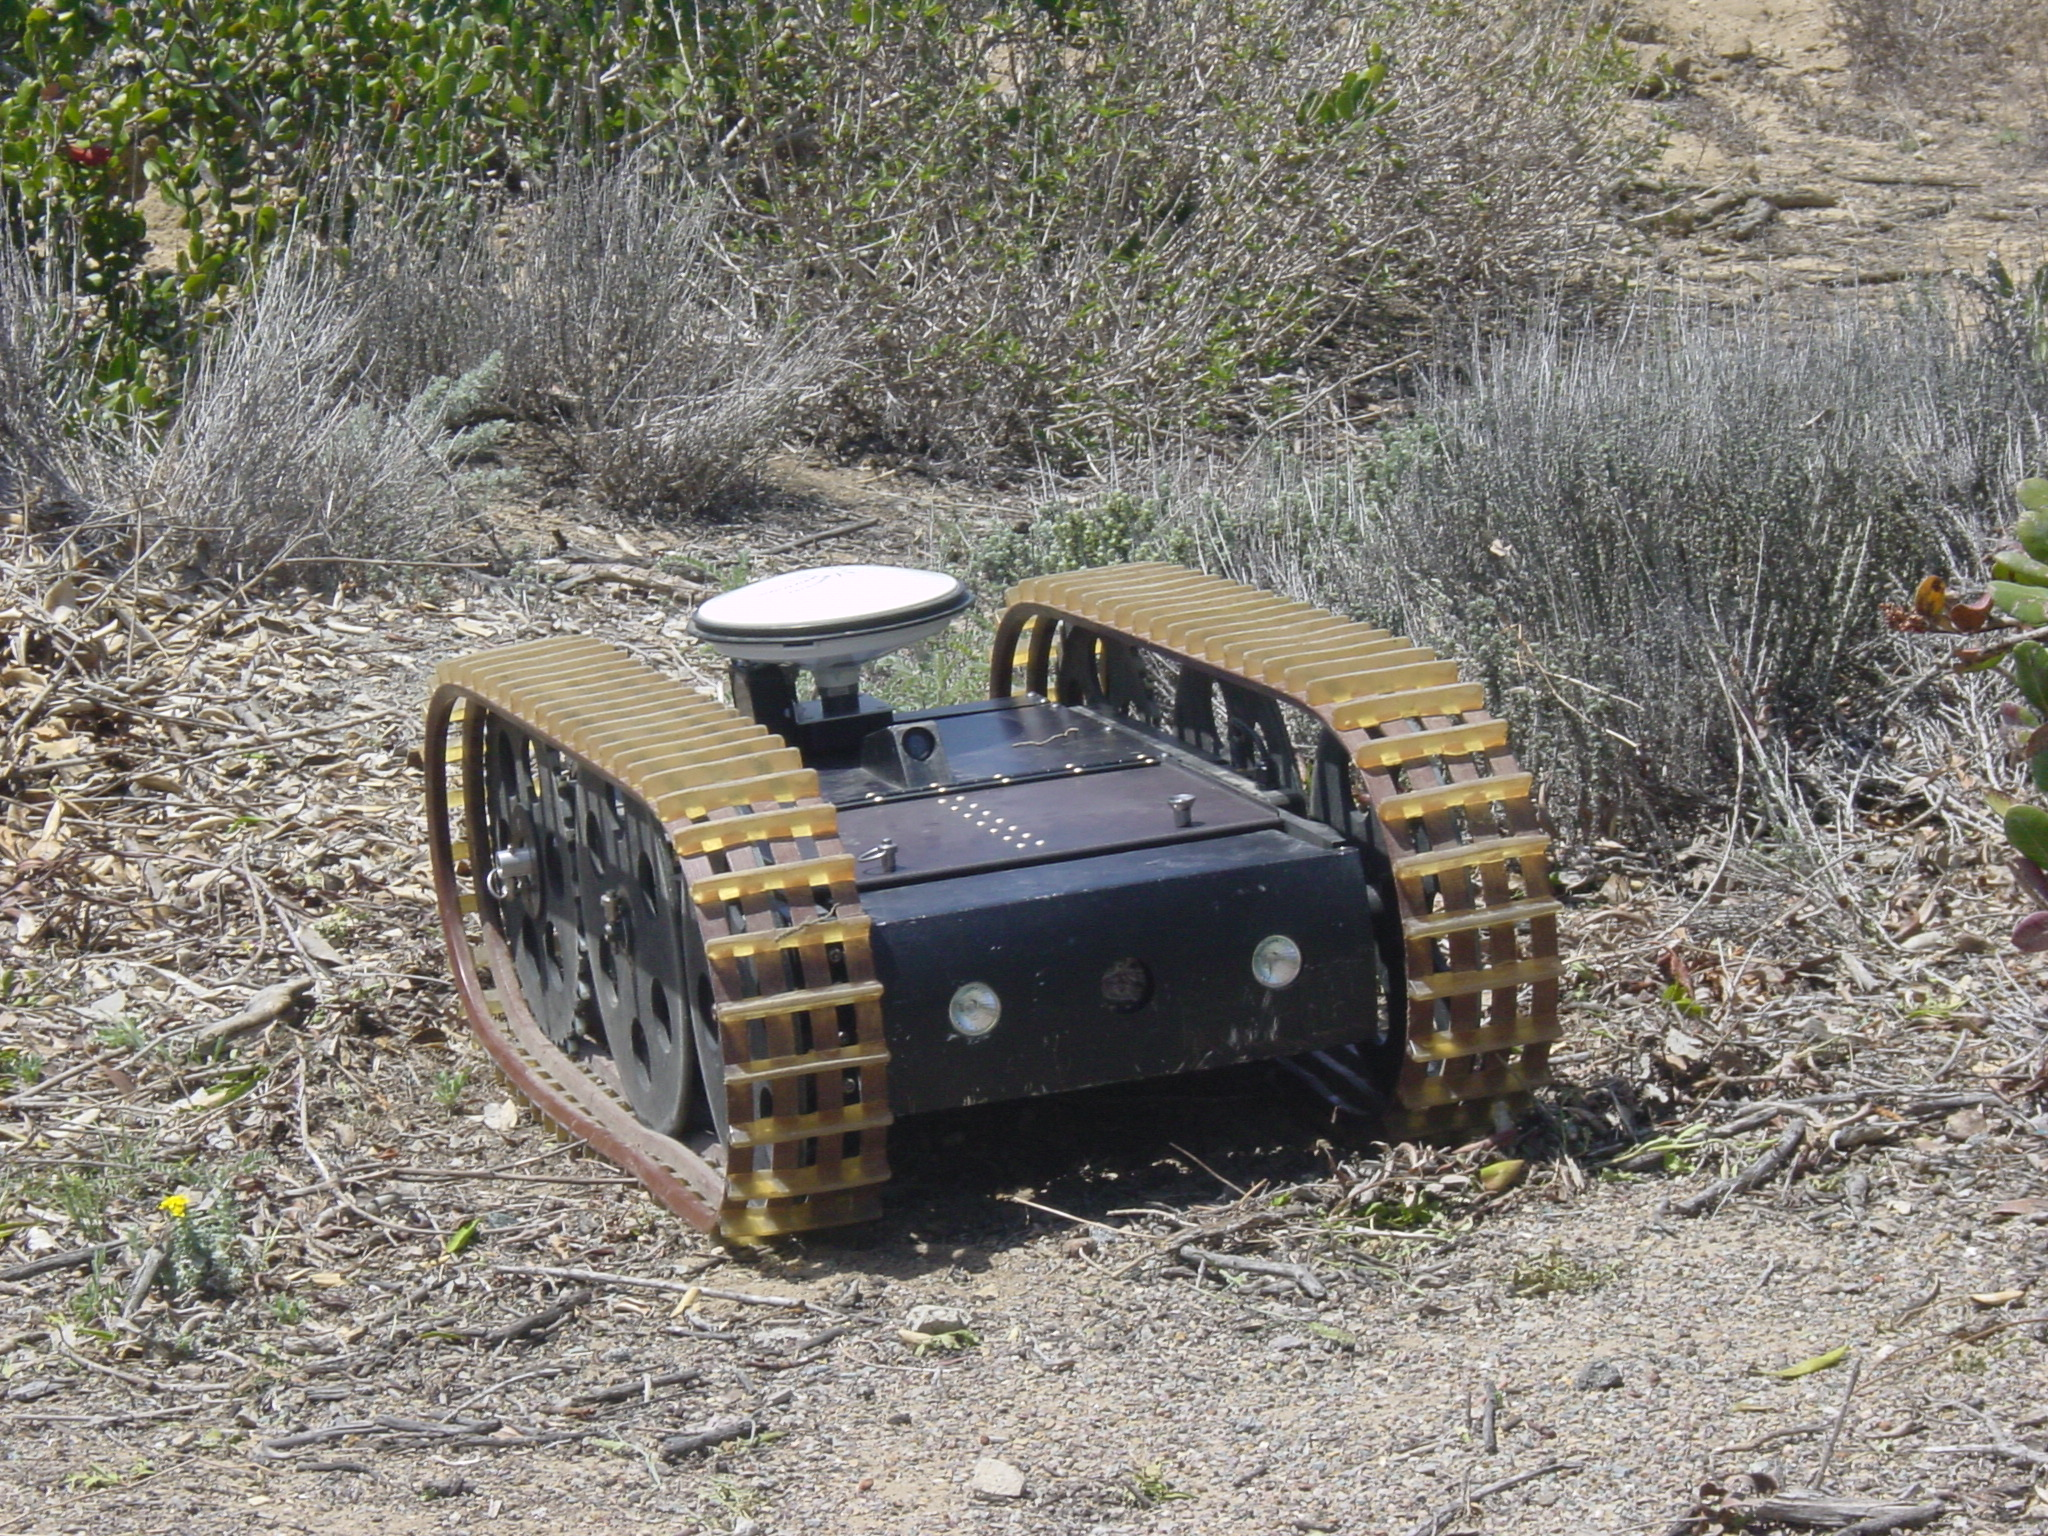
\includegraphics[width=.3\textwidth]{images/urbotWithGps}
	\caption{SSCPAC Urbot}
	\label{fig:urbot}
\end{figure}

The \href{http://www.autonomoussolutions.com/products/chaos.php}{Chaos} is manufactured by Autonomous Solutions and is shown in Figure \ref{fig:chaos}.

\begin{figure}[ht!]
	\centering
	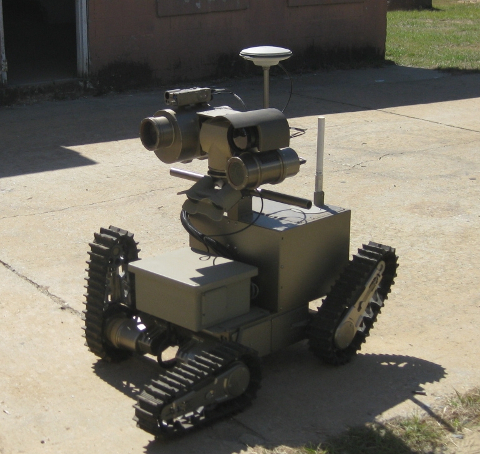
\includegraphics[width=.3\textwidth]{images/chaos}
	\caption{Autonomous Solutions Chaos}
	\label{fig:chaos}
\end{figure}

\section{MOCU \& JAUS}
\label{sec:mocujaus}
The Multi-Robot Operator Control Unit (MOCU), shown in Figure \ref{fig:mocu}, is a highly configurable front-end for simultaneous command and control of multiple systems and was created at SSCPAC \cite{PowellMOCU08}. MOCU has the ability to use a variety of communications protocols for interfacing to different systems and uses the Joint Architecture for Unmanned Systems (JAUS) protocol to send and receive data to all of the robots used in this research \cite{RoweJAUS08}. A combination of teleoperation using a joystick controller and autonomous navigation were used to collect data and test new ideas for estimation and controls. From within MOCU waypoints can be drawn on an overhead image of the operating area and from those waypoints a route is generated and downloaded to the robot using the JAUS protocol. The robot will then attempt to drive that route autonomously and send back status information to MOCU using the controls and estimation code that is the focus of this research.

\begin{figure}[ht!]
	\centering
	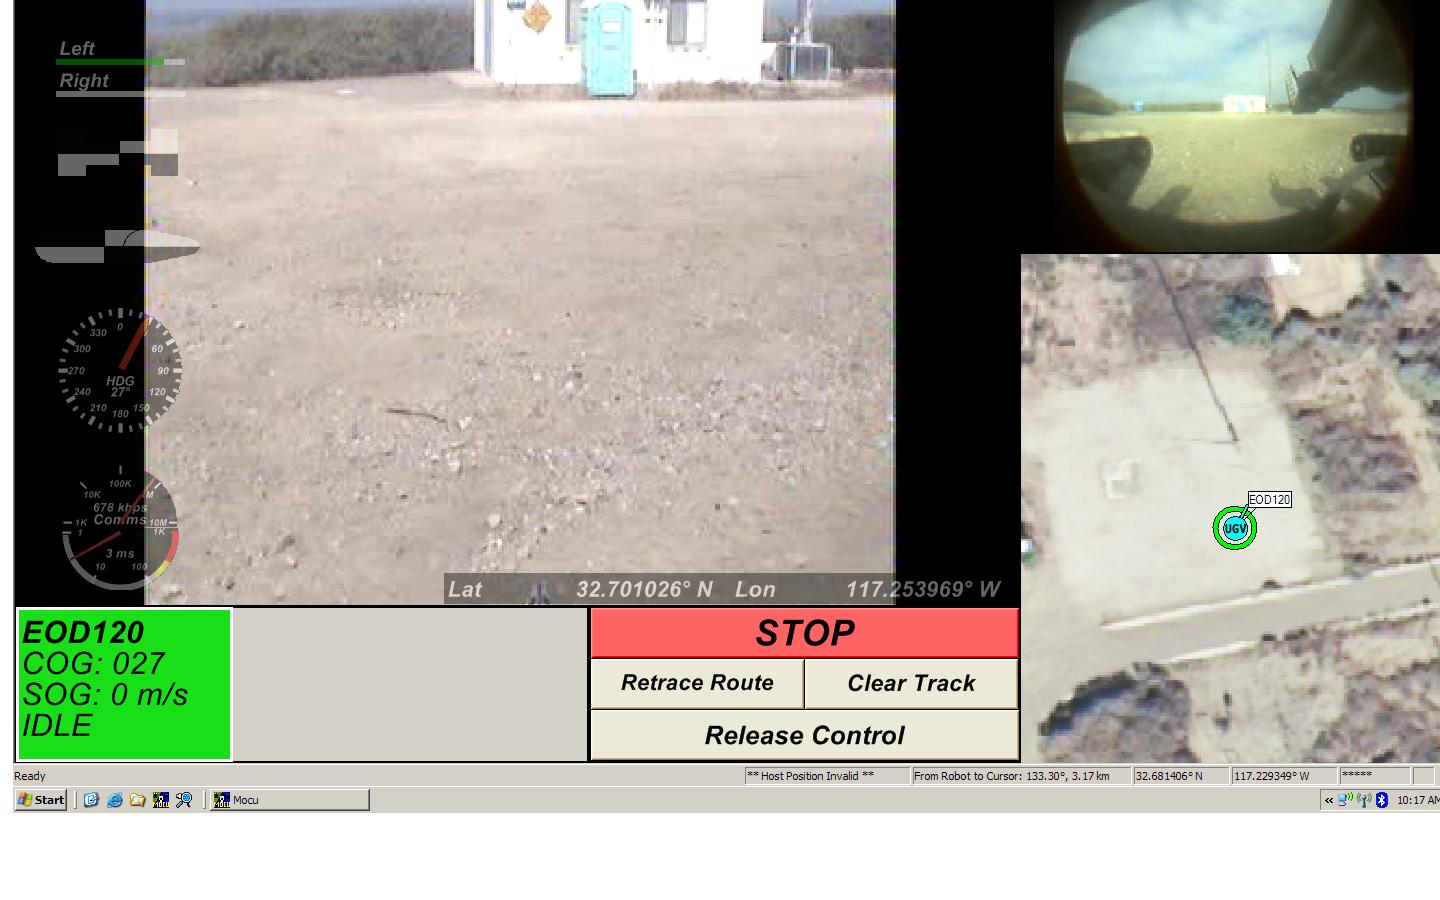
\includegraphics[width=.75\textwidth]{images/mocuPackbotScreenshot}
	\caption{Controlling Packbot with MOCU}
	\label{fig:mocu}
\end{figure}

\section{Sensors}
\label{sec:bgSensors}
The Packbot and Talon have their own computers that take in commands for desired linear and angular velocities. Those computers then output the correct motor controller commands that cause the robot to move at the desired velocities. Typically, the desired linear and angular velocity commands are generated by a user with a remote control. The research in this thesis was concerned with generating the velocity commands autonomously, or without human input, using a set of sensors installed in one of the payload bays of the robot.

For most of the results presented here the computer used for running the estimation and controls algorithms is the \href{http://www.beckhoff.com/english.asp?motherboards/cb4051.htm}{Beckhoff CB4051} with an Intel $2.0 GHz$ Core 2 Duo CPU. Tests were also conducted using an Intel Atom CPU as the payload computer with very similar results as obtained with the Core 2 Duo CPU.

The IMU in the payload bay is a \href{http://www.microstrain.com/3dm-gx1.aspx}{Microstrain 3DM-GX1} that outputs Euler angles and angular rates.

Two different GPS receivers were used on the robots. The GPS receiver used most often on all of the robots is a \href{http://www.novatel.com/products/gnss-receivers/oem-receiver-boards/oemv-receivers/}{Novatel OEMV}. Additionally, a \href{http://www.u-blox.com/gps-modules.html}{uBlox NEO-6Q} GPS receiver was used on both the Talon and Packbot during the course of experimentation. The Novatel receiver performed better overall, though the uBlox  was adequate. All of the results presented here use data from runs with the Novatel receiver.

A gyroscope is used to measure angular velocity of the robots. The \href{http://www.kvh.com/Commercial-and-OEM/Gyros-and-Inertial-Systems-and-Compasses/Gyros-and-IMUs-and-INS/Fiber-Optic-Gyros/DSP-3000.aspx}{KVH DSP-3000 Fiber Optic Gyro} is installed in the payload bay of all the robots tested here.

Originally, a compass was not used on the Packbot, but after initial testing it was determined that the heading reported by the Microstrain 3DM-GX1 was not very reliable and an \href{http://www.oceanserver-store.com/os3axdico3.html}{Ocean Server OS5000} compass was added to the payload bay. This compass gives outputs for pitch, roll and yaw angles. It was determined that the yaw angle output of this compass was not reliable enough to be used very often. Instead, a combination of integrating the KVH gyro output and, when available, the GPS yaw angle output, was used to generate the yaw angle estimate.

The Packbot and Talon are manufactured with wheel encoders that are read by the main computer and used to calculate the linear and angular velocities of the robot. The payload computer has access to these values when communicating with the main computer. Initially, the wheel encoder data was not being used so that backwards compatibility with other small robots without wheel encoders would be maintained. However, the systems without wheel encoders are no longer used by EOD groups, so the wheel encoder data has been incorporated into the sensor suite used by the algorithms in this thesis.

\section{Estimation and Control Software}
\label{sec:bgSoftware}
The SSCPAC robotics group has developed the Autonomous Capabilities Suite (ACS) which incorporates many different robotics related algorithms into a single software package that can be run on a wide variety of robots. ACS is able to easily accomodate different payload and sensor suites \cite{Sights06}. The Kalman filter implementation was done in ACS.

A JAUS library written by SSCPAC provides for communications between the robots and MOCU.

The original path planning and controls software was written by SSCPAC for the Man Portable Robotic Systems (MPRS) program \cite{Bruch02} and extended for use on unmanned surface vehicles \cite{Ebken05}, \cite{Larson06}, \cite{Larson07}. The new model-based controller is implemented in the MPRS code and will be ported to ACS in the near future.

A single program was built by combining the ACS Kalman filter code, the JAUS library and the MPRS code. This is the program that was run for all of the experiments presented here.
